\documentclass[12pt]{article}\usepackage[]{graphicx}\usepackage[]{color}
%% maxwidth is the original width if it is less than linewidth
%% otherwise use linewidth (to make sure the graphics do not exceed the margin)
\makeatletter
\def\maxwidth{ %
  \ifdim\Gin@nat@width>\linewidth
    \linewidth
  \else
    \Gin@nat@width
  \fi
}
\makeatother

\definecolor{fgcolor}{rgb}{0.345, 0.345, 0.345}
\newcommand{\hlnum}[1]{\textcolor[rgb]{0.686,0.059,0.569}{#1}}%
\newcommand{\hlstr}[1]{\textcolor[rgb]{0.192,0.494,0.8}{#1}}%
\newcommand{\hlcom}[1]{\textcolor[rgb]{0.678,0.584,0.686}{\textit{#1}}}%
\newcommand{\hlopt}[1]{\textcolor[rgb]{0,0,0}{#1}}%
\newcommand{\hlstd}[1]{\textcolor[rgb]{0.345,0.345,0.345}{#1}}%
\newcommand{\hlkwa}[1]{\textcolor[rgb]{0.161,0.373,0.58}{\textbf{#1}}}%
\newcommand{\hlkwb}[1]{\textcolor[rgb]{0.69,0.353,0.396}{#1}}%
\newcommand{\hlkwc}[1]{\textcolor[rgb]{0.333,0.667,0.333}{#1}}%
\newcommand{\hlkwd}[1]{\textcolor[rgb]{0.737,0.353,0.396}{\textbf{#1}}}%

\usepackage{framed}
\makeatletter
\newenvironment{kframe}{%
 \def\at@end@of@kframe{}%
 \ifinner\ifhmode%
  \def\at@end@of@kframe{\end{minipage}}%
  \begin{minipage}{\columnwidth}%
 \fi\fi%
 \def\FrameCommand##1{\hskip\@totalleftmargin \hskip-\fboxsep
 \colorbox{shadecolor}{##1}\hskip-\fboxsep
     % There is no \\@totalrightmargin, so:
     \hskip-\linewidth \hskip-\@totalleftmargin \hskip\columnwidth}%
 \MakeFramed {\advance\hsize-\width
   \@totalleftmargin\z@ \linewidth\hsize
   \@setminipage}}%
 {\par\unskip\endMakeFramed%
 \at@end@of@kframe}
\makeatother

\definecolor{shadecolor}{rgb}{.97, .97, .97}
\definecolor{messagecolor}{rgb}{0, 0, 0}
\definecolor{warningcolor}{rgb}{1, 0, 1}
\definecolor{errorcolor}{rgb}{1, 0, 0}
\newenvironment{knitrout}{}{} % an empty environment to be redefined in TeX

\usepackage{alltt}
\usepackage[margin=1in]{geometry}
\usepackage{setspace}
\doublespacing
% \usepackage{fullpage}
%\usepackage{graphicsx}
% \usepackage[colorlinks=true,linkcolor=blue]{hyperref}
\usepackage[backend=bibtex,style=authoryear]{biblatex}
\addbibresource{MosqBiblio.bib}
%For regular papers, a motivating example should be presented early in the paper. The statistical development should then be presented, and the results applied to the example.
\title{A method for identifying households at high risk for mosquito borne illnesses.}
\date{}
\IfFileExists{upquote.sty}{\usepackage{upquote}}{}
\begin{document}
\maketitle







\section{Abstract}
Mosquito borne illnesses are a significant threat to public health. Concerted efforts have been made in the past decade to reduce and in some cases eliminate mosquito borne diseases with the use of prophylactic interventions. The World Health Organization recommends preferential administration of interventions to those with the highest risk of negative/ severe health outcomes. However,  previous research has also identified the benefit of additionally targeting interventions at those with the highest risk of infections to prevent subsequent transmission. We develop a methodology that combines these two targets of health outcomes and infection risk. We use census information to determine health risk and we use a topographic wetness index as an indicator of habitat for mosquito species that inhabit natural environments.  We implement the method to evaluate the community-reported administration of interventions at two sites in Kenya. We find preferential administration of interventions at the high-elevation epidemic-prone site but not at the low-elevation endemic site. Our results have important implications for assessing the administration of interventions in the battle against mosquito borne illnesses.

\textbf{Keywords:} Malaria, West Nile Virus, GIS, Remote Sensing, Public Health 

\section{Introduction}
%introduce the problem
Malaria and other mosquito borne illnesses are considered a significant threat to public health and a socio-economic burden in countries where these diseases are either endemic or epidemic (\cite{Crouch}). Concerted efforts have been made in the past decade to reduce and in some cases eliminate malaria specifically. Many national strategic plans to reduce or eliminate malaria are in their third generation.  The World Health Organization recommends prioritizing the administration of interventions to pregnant women and young children followed by progressively achieving intervention coverage of all community members. The preferential administration of interventions to pregnant women and young children reflects the disproportionate disease burden borne by this group and the increased likelihood of severe health outcomes(\cite{Bousema2012}). However,  previous research has identified the benefit of additionally targeting interventions at those with the highest risk of infections (\cite{Schantz-Dunn2009}). Identifying individuals which are both vulnerable to disease and likely to be exposed to an infected mosquito is therefore a priority.  However, identifying high risk individuals can be costly and inefficient.\\

The Topographic Wetness Index (TWI) (\cite{Beven1979}) derived from freely available remotely-sensed topographic data has been previously investigated as a tool for assessing risk of malaria infection (\cite{Cohen2008,Cohen2010}). TWI can potentially identify areas where water is likely to pool and \emph{Anopheles} densities are likely to be higher. This method, therefore, has the potential to both inform new distribution campaigns and evaluate the efficacy of existing campaigns.  However, traditional TWI algorithms are complicated and generally require specialized software to implement.  Moreover, simply identifying areas where mosquitoes are likely to breed does not account for the differential health risk of the exposed population.  We develop a simple, matrix-based, methodology using topographic data and combine this with a household census of demographics to identify high risk households.  We apply the method to two sites in Kenya where malaria is either endemic or epidemic-prone.  We compare our methodology to a traditional Topographic  Wetness Index using data on intervention use for two interventions at two sites in Kenya. \\%This method, therefore, has the potential to both inform new distribution campaigns and evaluate the efficacy of existing campaigns.



\section{Statistical Methodology}%main idea is to use traditional or aspect variance methods and see if there is a substantial difference.  Would be best 
Every household on a landscape will vary with respect to both the risk of exposure to mosquitoes and the number of at risk individuals in the household. We develop a method to combine these two risk factors into an overall risk score for each household within a management area in order to identify the households which will yield the greatest benefit from the application of limited resources.\\

\subsection{Topographical Wetness Index}

The Topographical Wetness index was originally introduced by Beven and Kirby in 1979 (\cite{Beven1979}).  TWI combines a measure of the amount of upstream drainage area with the local slope to determine the amount of wetness likely to accumulate at a point and is defined by Beven and Kirby generally as:
$$ln\frac{a}{tanb},$$
where $a$ is the local up-slope area (local area draining to the point) and $tanb$ is the local slope in radians.  The TWI is designed to predict the amount of water that is likely to flow into an area, based on surface topology, and the rate at which this water will flow out of an area.  Since TWI was first defined numerous methods have been developed to calculate it and several review papers have been published (\cite{Quinn1995,Sørensen2006}) as well as alternative modeling strategies developed (\cite{Grabs2009}).  Areas with high in-flow and low out-flow are likely provide habitat for breeding mosquitoes. \\

The primary goal of using TWI in this application is to identify areas where mosquitoes are likely to lay their eggs and go through the immature stages of the life-cycle.  However, the general TWI was originally designed to model surface water flow and not necessarily to identify areas where water will pool. A simpler algorithm for identifying only areas where water is likely to pool may perform as well, or better, than a general TWI algorithm and would not require specialized GIS software for implementation.  To examine this, we implement 2 different algorithms which differ in their calculation of the up-slope area and local slope: 1) the SAGA Wetness Index (\cite{Bohner2002}) (hereafter "general TWI"), and 2) a simplified topographic wetness index which simply identifies depressions without regard to up-slope area (hereafter "restricted TWI").  \\


We carried out all analyses using the statistical programming language R version 3.2.3 (\cite{RCoreTeam2015}), with the exception of the SAGA TWI which was calculated with the SAGA open-source GIS software (\cite{Bohner2006}).  Details for calculation of the general TWI are available in the software documentation available at http://www.saga-gis.org (\cite{Conrad2015}).  The method involves, for every point on the landscape:  calculating the up-slope area from which water will flow to the point,  calculating the catchment area, and the slope of the catchment area.  Areas with a larger up-slope area and a smaller catchment area slope are predicted to have more water accumulation.\\

In contrast to the relatively complicated calculation of a general TWI, we suggest a simple model based on identifying depressions with low outflow and disregarding the up-slope area.  We first identify depressions and valleys by identifying pixels which are lower than the average of their neighbors.  We do this by first calculating the average elevation of the surrounding pixels for each pixel ($p$) in the landscape at three resolutions of increasing size:  

$$\mu_{i,j} = \frac{\sum_{p \in j}e_p}{|p \in j|},$$

where $\mu_{i,j}$ is the average elevation of the pixels in the window of size $j$ surrounding pixel $i$.  The size of the windows is somewhat arbitrary but the idea is to identify small depressions from large ones so we suggest $90m \times 90m$, $210m \times 210m$, and $330m \times 330m$.  These sizes may be adjusted or tuned to a particular landscape if information is available to do so.  We then subtract the mean elevation from the actual elevation at each pixel from the three calculated averages and sum these differences.\\

$$\delta e_{i,j} = e_i - \mu_{i,j} $$
$$\Delta e_{i} = \sum_{j \in 1,2,3} \delta e_{i,j}$$

We then identify areas with low outflow by calculating the variance of the aspects (direction the slope faces) of neighboring pixels, $\theta$.  Since aspect is measured on a circular scale from 1 to 360 the variance of two aspects which are in fact quite close to each other but on opposite sides of the circular scale reset at 360 would be artificially high.  For example, the aspect of two points facing close to due north could be 359 and 1.  The variance of these two points would be $var(359,1)= 64082$.  However, the variance of two aspects of equal distance but not on opposite sides of the circular reset would be $var(1,3) = 2$.  In order to mitigate this difficulty we first translate each aspect to a cardinal direction denoted 1, 2, 3, or 4. We then calculate the variance of the aspects of the cells in each of 3 moving windows the same size as above ($90m \times 90m$, $210m \times 210m$, and $330m \times 330m$) and sum the resulting variances for each pixel:

$$\theta_{i} = \sum_{j \in 1,2,3} var(a_{i \in j}),$$

where $a_{i \in j}$ are the set of aspects in the moving window $j$  around pixel $i$.  The final wetness index is then calculated as, 
$$w_i = -1 \times \Delta e_i \times \theta_i.$$

Relatively large positive values of $w_i$ are expected to have higher wetness than small positive numbers.  Negative numbers indicate a ridge or peak and are therefore expected to be dry.\\
 

We assign each household a risk for exposure to mosquitoes (exposure risk hereafter) by deriving a continuous risk surface over the study area from each TWI algorithm.  We assume the mosquito exposure risk of a household is inversely related to the distance to one or more of these high-wetness areas.  Therefore,  we apply a Gaussian filter with $\sigma = 10$ to create a weighted average of mosquito risk for each cell in the study area.  The Gaussian filter is an isometric 2-dimensional smoothing function with a Gaussian kernel.  The value of $\sigma$ determines the degree of smoothing and should be scaled appropriately to match the resolution of the data.  The value of $\sigma$ can be tuned for a specific application if data is available and appropriate to do so. Each house is then assigned the risk score of the cell it is in or, for high resolution topographical data such as LiDAR (laser radar), the average of the cells a property occupies.\\


\subsection{Individual Health Risk}
Each household varied with respect to both the risk of exposure to mosquitoes and the number of at-risk individuals in the household. The household risk formulas will vary depending on the disease under study and the most vulnerable population(s) for that disease.  We recommend a simple additive risk score, like the score formula provided below developed for malaria, based on expert opinion or relevant literature. The sole purpose of the health risk score is to differentiate households with high risk from those with low risk.  More complicated formulas can be constructed but we believe a simple formula will be easier to interpret and adequate for most applications.\\

\subsection{Overall Risk}

To be at risk for a poor outcome a person must 1) come in contact with a disease harboring mosquito,  and 2) be inherently vulnerable to infection (e.g. very young or pregnant).  We create two risk scores representing each of these types of risk for every household on the landscape.  Since these risks will be calculated on different scales we center at 0 and standardize risk scores so that they are scale-independent.  These two scores can then be combined with a weighted sum to create an overall risk score for the household.  Weights in the sum are determined by expert opinion, in our example below we use equal weights.  This method lends itself well to the addition of additional risk scores, such as the distance to a health care provider, or even risk attenuating factors such as the presence of window screens, which can all be summed together with appropriate weights. 









\subsection{Example Analysis}

%Example Application
The government of Kenya developed the “National Malaria Strategy 2009-2017” in response to the ongoing threat of malaria (\cite{Ministryofpublichealthandsanitation2009}). This strategy outlined 6 objectives,  the first of which is “to have at least 80\% of people living in malaria risk areas using appropriate malaria preventive interventions.” The two primary non-pharmaceutical interventions identified in the plan are Indoor Residual Spraying (IRS) and Long Lasting Insecticidal Nets (LLINs). The strategy outlined for achieving the intervention objective included the initial mass distribution of LLINs where malaria is either endemic (western lowlands) or epidemic-prone (western highlands); followed by routine distribution of LLINs to pregnant women and children under 1 year of age and a subsidized sale of LLINs. The strategy also outlined the use of widespread IRS followed by focal treatments in epidemic-prone areas, i.e. areas where mosquitoes are likely to breed.  We use this information to evaluate our methodology.\\

% The World Health Organization recommends prioritizing the administration of interventions to pregnant women and young children followed by progressively achieving intervention coverage of all community members. The preferential administration of interventions to pregnant women and young children reflects the disproportionate disease burden borne by this group (\cite{Bousema2012}). However,  previous research has identified the benefit of additionally targeting interventions at those with the highest risk of infections (\cite{Schantz-Dunn2009}). Identifying individuals which are both vulnerable to infection and likely to be exposed to an infected mosquito is therefore a priority.  However, existing distribution campaigns do not typically account for both infection risk and disease burden simultaneously.\\

Prior to the initiation of a community-based research program,  two study sites in western Kenya were mapped and a census was taken. These two sites represent the western highland (hereafter “epidemic-prone”,  N = 3380) and lowland (hereafter “endemic”,  N = 604) populations. Our objective was to determine if the highest risk households were given preference in the administration of interventions in the form of both bed nets and indoor residual spraying.\\

We collected demographic information for each occupant including age and sex. Both sites have had partial treatment with both LLINs and IRS and household heads provided initial information about LLIN ownership and government administration of household IRS in the previous six months.  We assigned an individual-based health risk score (health risk hereafter) to each household with the following formula:

$$Health\ Risk\ Score  =  (2 \times \ Children\ \leq 1) + (1 < \ Children\  \leq 5) + (2 \times \ Pregnant\ Women)$$

We assigned twice the weight to children under 1 and pregnant women since they have been previously identified as high risk (\cite{Gupta1999, Snow1999, Menendez2000}).  This formula is tailored for malaria exposure but can be adjusted based on \emph{a priori} information about the individual risks for a particular mosquito borne disease. For example, for the West Nile virus those of age 65 years and older may have an increased. risk of neurological symptoms and permanent neural damage.\\

We added the standardized household health risk with the standardized household exposure risk to create a combined risk.  We then determined if high risk households are more likely to have received either a bed-net or indoor residual spraying with a logistic model;

$$log(\frac{p}{1-p}) = \beta_0 + \beta_1 \times \ Combined\ Household\ Risk, $$

where $p$  =  Probability of a house having a treatment.  If $e^{\beta_1}$ is $>$ 1 and statistically significant ($\alpha = 0.05$) then high-risk households are more likely to receive treatment.  %We used a restricted cubic spline function to determine if there was a linear relationship between the log odds of treatment and combined risk.  
We modeled the high and low sites separately because these sites differed substantially in topography, level of malaria transmission, and intervention administration protocols.  We also modeled the two interventions separately since they are administered under different protocols.  Finally, in order to examine the utility of each TWI algorithm, we repeated the analysis using both the general and restricted TWI.\\  %If we found evidence of a non-linear relationship we categorized the risk score into quartiles and re-fit with a means model. 




























\subsection{Results}
The odds of receiving either a bed net or indoor residual spraying were higher for households with higher combined risk,  but only at the high site (\ref{ORcmb}).  For each 1 standard deviation increase in combined risk at the high site the probability of receiving a bed net increased 27\% (OR: 1.27,  95\% CI: 1.18,  1.35) and the probability of indoor residual spraying increased 15\% (OR: 1.15,  95\% CI: 1.03,  1.29).  At the low site,  we found no preferential administration of either treatment to high combined risk households.  We found some evidence,  from the fitting of a restricted cubic spline,  of a non-linear relationship between the log-odds of net use and combined risk at the low site.  However,  accounting for non-linearity in the model did not change the results so we only report the linear model here.\\ 

The probability of bed net use at the high site was more strongly associated with health risk,  whereas the probability of indoor residual spraying at the high site was more strongly associated with exposure risk (\ref{ORtrt}).  However,  We did not find the same pattern at the low site where we found households with high exposure risk were actually significantly less likely to receive indoor residual spraying (OR: 0.35,  95\% CI: 0.14,  0.83).  \\



\begin{table}[ht]
\centering
\begin{tabular}{lllll}
  \hline 
Site & Treatment & OR & Lower 95\% CI & Upper 95\% CI \\ 
  \hline
High & Net & 1.35 & 1.26 & 1.44 \\ 
   & Spray & 1.13 & 1.00 & 1.26 \\ 
  Low & Net & 1.09 & 0.86 & 1.39 \\ 
   & Spray & 0.9 & 0.61 & 1.34 \\ 
   \hline
\end{tabular}
\caption{Odds of receiving a treatment as a function of combined risk.} 
\label{ORcmb}
\end{table}





\begin{table}[ht]
\centering
\begin{tabular}{llllllll}
  \hline
 &  & \multicolumn{3}{l}{Health Risk} & \multicolumn{3}{l}{Exposure Risk}  \\ 
  
Site & Treatment & OR & Lower 95\% CI & Upper 95\% CI & OR & Lower 95\% CI & Upper 95\% CI \\ 
 \hline
  High & Net & 1.36 & 1.27 & 1.45 & 1.01 & 0.93 & 1.10 \\ 
   & Spray & 1.08 & 0.96 & 1.22 & 1.32 & 1.14 & 1.53 \\ 
  Low & Net & 1.21 & 0.94 & 1.55 & 0.58 & 0.31 & 1.10 \\ 
   & Spray & 1.08 & 0.67 & 1.74 & 0.34 & 0.15 & 0.79 \\ 
   \hline
\end{tabular}
\caption{Odds of treatment from risk of either mosquito exposure or malaria risk.} 
\label{ORtrt}
\end{table}





















\subsection{Restricted TWI}

The use of the restricted TWI algorithm identified fewer regions as high risk than the general TWI at both sites and was less likely to assign exposure risk to areas near a channel (Fig. \ref{twis}).  The use of the restricted TWI based risk surface in the combined risk score increased the odds of a high-risk labelled household to have received a treatment for both the high and low sites,  although the increase in OR for the low site remained non-significant (Table \ref{Sens}).

  


\begin{table}[ht]
\centering
\begin{tabular}{llllllll}
  \hline
 &  & \multicolumn{3}{l}{General TWI} & \multicolumn{3}{l}{Restricted TWI}\\
Site & Treatment & OR & Lower 95\% CI & Upper 95\% CI & OR & Lower 95\% CI & Upper 95\% CI \\ 
  \hline
High & Net & 1.35 & 1.26 & 1.44 & 1.45 & 1.33 & 1.59 \\ 
   & Spray & 1.13 & 1.00 & 1.26 & 1.22 & 1.05 & 1.42 \\ 
  Low & Net & 1.09 & 0.86 & 1.39 & 1.33 & 0.93 & 1.90 \\ 
   & Spray & 0.90 & 0.61 & 1.34 & 1.10 & 0.59 & 2.03 \\ 
   \hline
\end{tabular}
\caption{Comparison of results when constructing combined risk from the restricted TWI or general TWI.} 
\label{Sens}
\end{table}

\begin{figure}
\centering
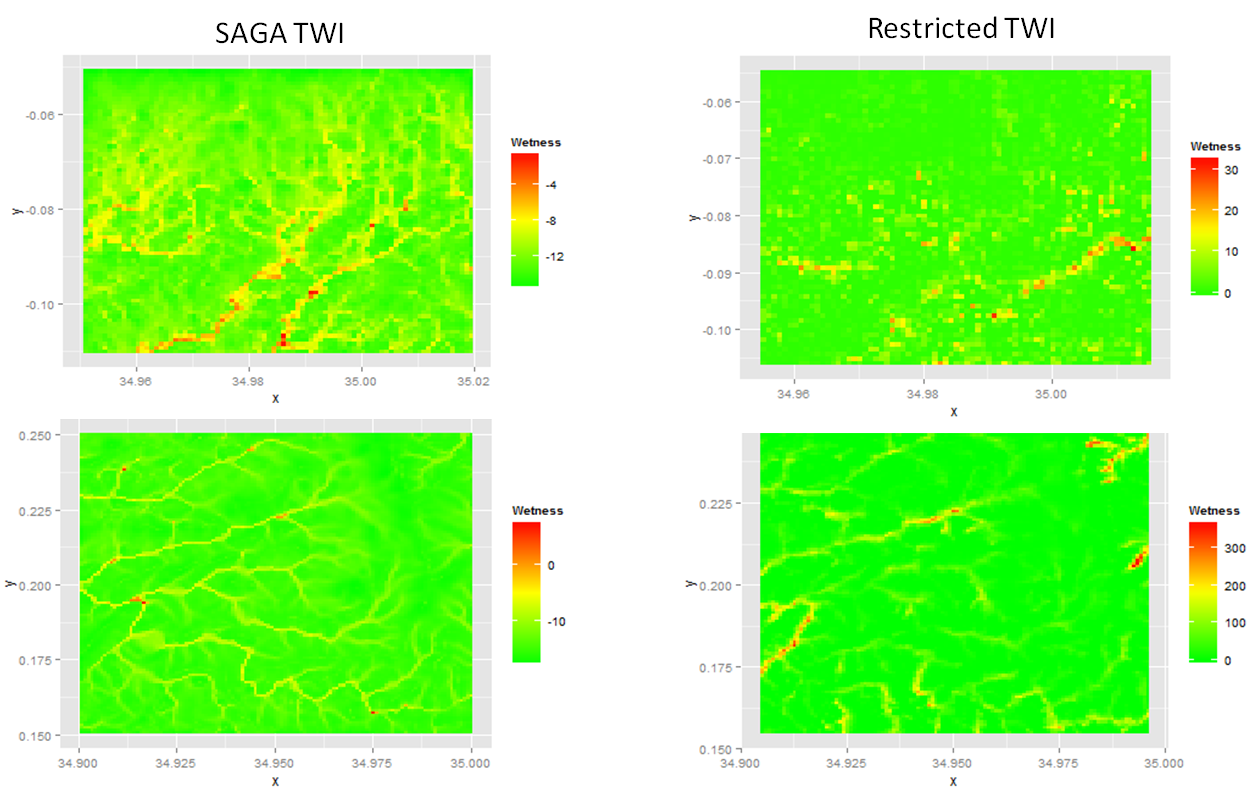
\includegraphics[scale=.5]{./figure/CompareTWI.png}
\caption{Comparison of the general TWI (left) and the restricted TWI (right) showing the lower extent of channels identified as moderate to high risk by the restricted TWI.  The restricted TWI also identified several areas missed by the general TWI. }
\label{twis}
\end{figure}



%Table 4.  Comparison of the odds of receiving a treatment based on health risk due to age with and without the inclusion of elderly household members. 


\section{Discussion}
Our methodology is motivated by the need to improve the efficiency of intervention administration protocols and evaluate existing protocols.  Our example analysis evaluates existing protocols in which the administration of bed nets target pregnant women.  Therefore,  we would expect that households with young children would be more likely to have LLINs.  We found that health risk was associated with an increased probability of LLIN use at the high site but not the low site.  Similarly, under current protocols, indoor residual spraying is intended to target households at high risk for mosquito exposure  so we would expect that households with high exposure risk would be associated with indoor residual spraying.  Again,  this is the pattern we observed at the high site but not the low site where we found the opposite association.\\

Since we do not have mosquito incidence data we evaluate the efficacy of each TWI algorithm by how closely each algorithm matches our expectations based on the intervention administration protocol at each site.  The general TWI algorithm identified channels at both sites as moderate to high risk.  However, while these channels are likely to have higher wetness, the water may drain too quickly to provide quality breeding habitat for mosquitoes.  Use of the restricted TWI algorithm identified fewer channels as having moderate to high exposure risk while identifying some areas not identified by the general TWI algorithm (Fig. \ref{twis}).  Therefore, the restricted TWI algorithm may out-perform the general TWI in identifying mosquito breeding sites.  Our results comparing both TWI algorithms indicates a stronger association between the restricted TWI and intervention use indicating better alignment between the restricted TWI and mosquito risk assessments on the ground. This was particularly noticeable when evaluating the OR of a household receiving indoor residual spraying at the low site where the association was at least in the preferable direction, albeit not significantly.  We believe our method can be used to quickly evaluate the overall risk for a given household and improve the efficiency of distribution protocols.\\

Our method does not depend on accurately identifying the absolute risk of any given household, but rather the relative risk of every household on the landscape.  This is important when trying to determine which areas should be targeted when resources are limited, as is often the case in areas where mosquito-borne diseases are transmitted. We believe the restricted TWI described in appendix A provides a simple and easily implemented algorithm for identifying high risk areas which may perform better than more complicated TWI algorithms based on the calculation of up-slope areas.  However, the sensitivity of our results to choice of TWI algorithm suggests that the TWI should be validated with additional information such as infection data.  This has been done previously (\cite{Cohen2008, Cohen2010}),  but only with a single algorithm at a single site.  We recommend further evaluation of TWI algorithms with actual mosquito borne infection information at multiple sites, preferably with different topographies.\\


\printbibliography


\end{document}
